El nivel regulatorio constituye el sistema de control en tiempo real del robot, gestionando directamente actuadores y sensores mediante ejecución de comandos recibidos desde el nivel supervisor.

El firmware se estructura en tres capas jerárquicas que separan responsabilidades según nivel de abstracción, como se muestra en la Figura \ref{fig:arquitectura_regulatorio}:

\begin{itemize}[label=$\bullet$]
\item \textbf{Capa de controladores de hardware (drivers):} Interactúa directamente con periféricos del microcontrolador mediante registros y temporizadores
\item \textbf{Capa de control de movimiento:} Implementa generación de trayectorias mediante perfiles de velocidad y coordinación de ejes
\item \textbf{Capa de aplicación:} Proporciona interfaz de alto nivel para comandos del sistema supervisor mediante protocolo UART
\end{itemize}

\begin{figure}[H]
    \centering
    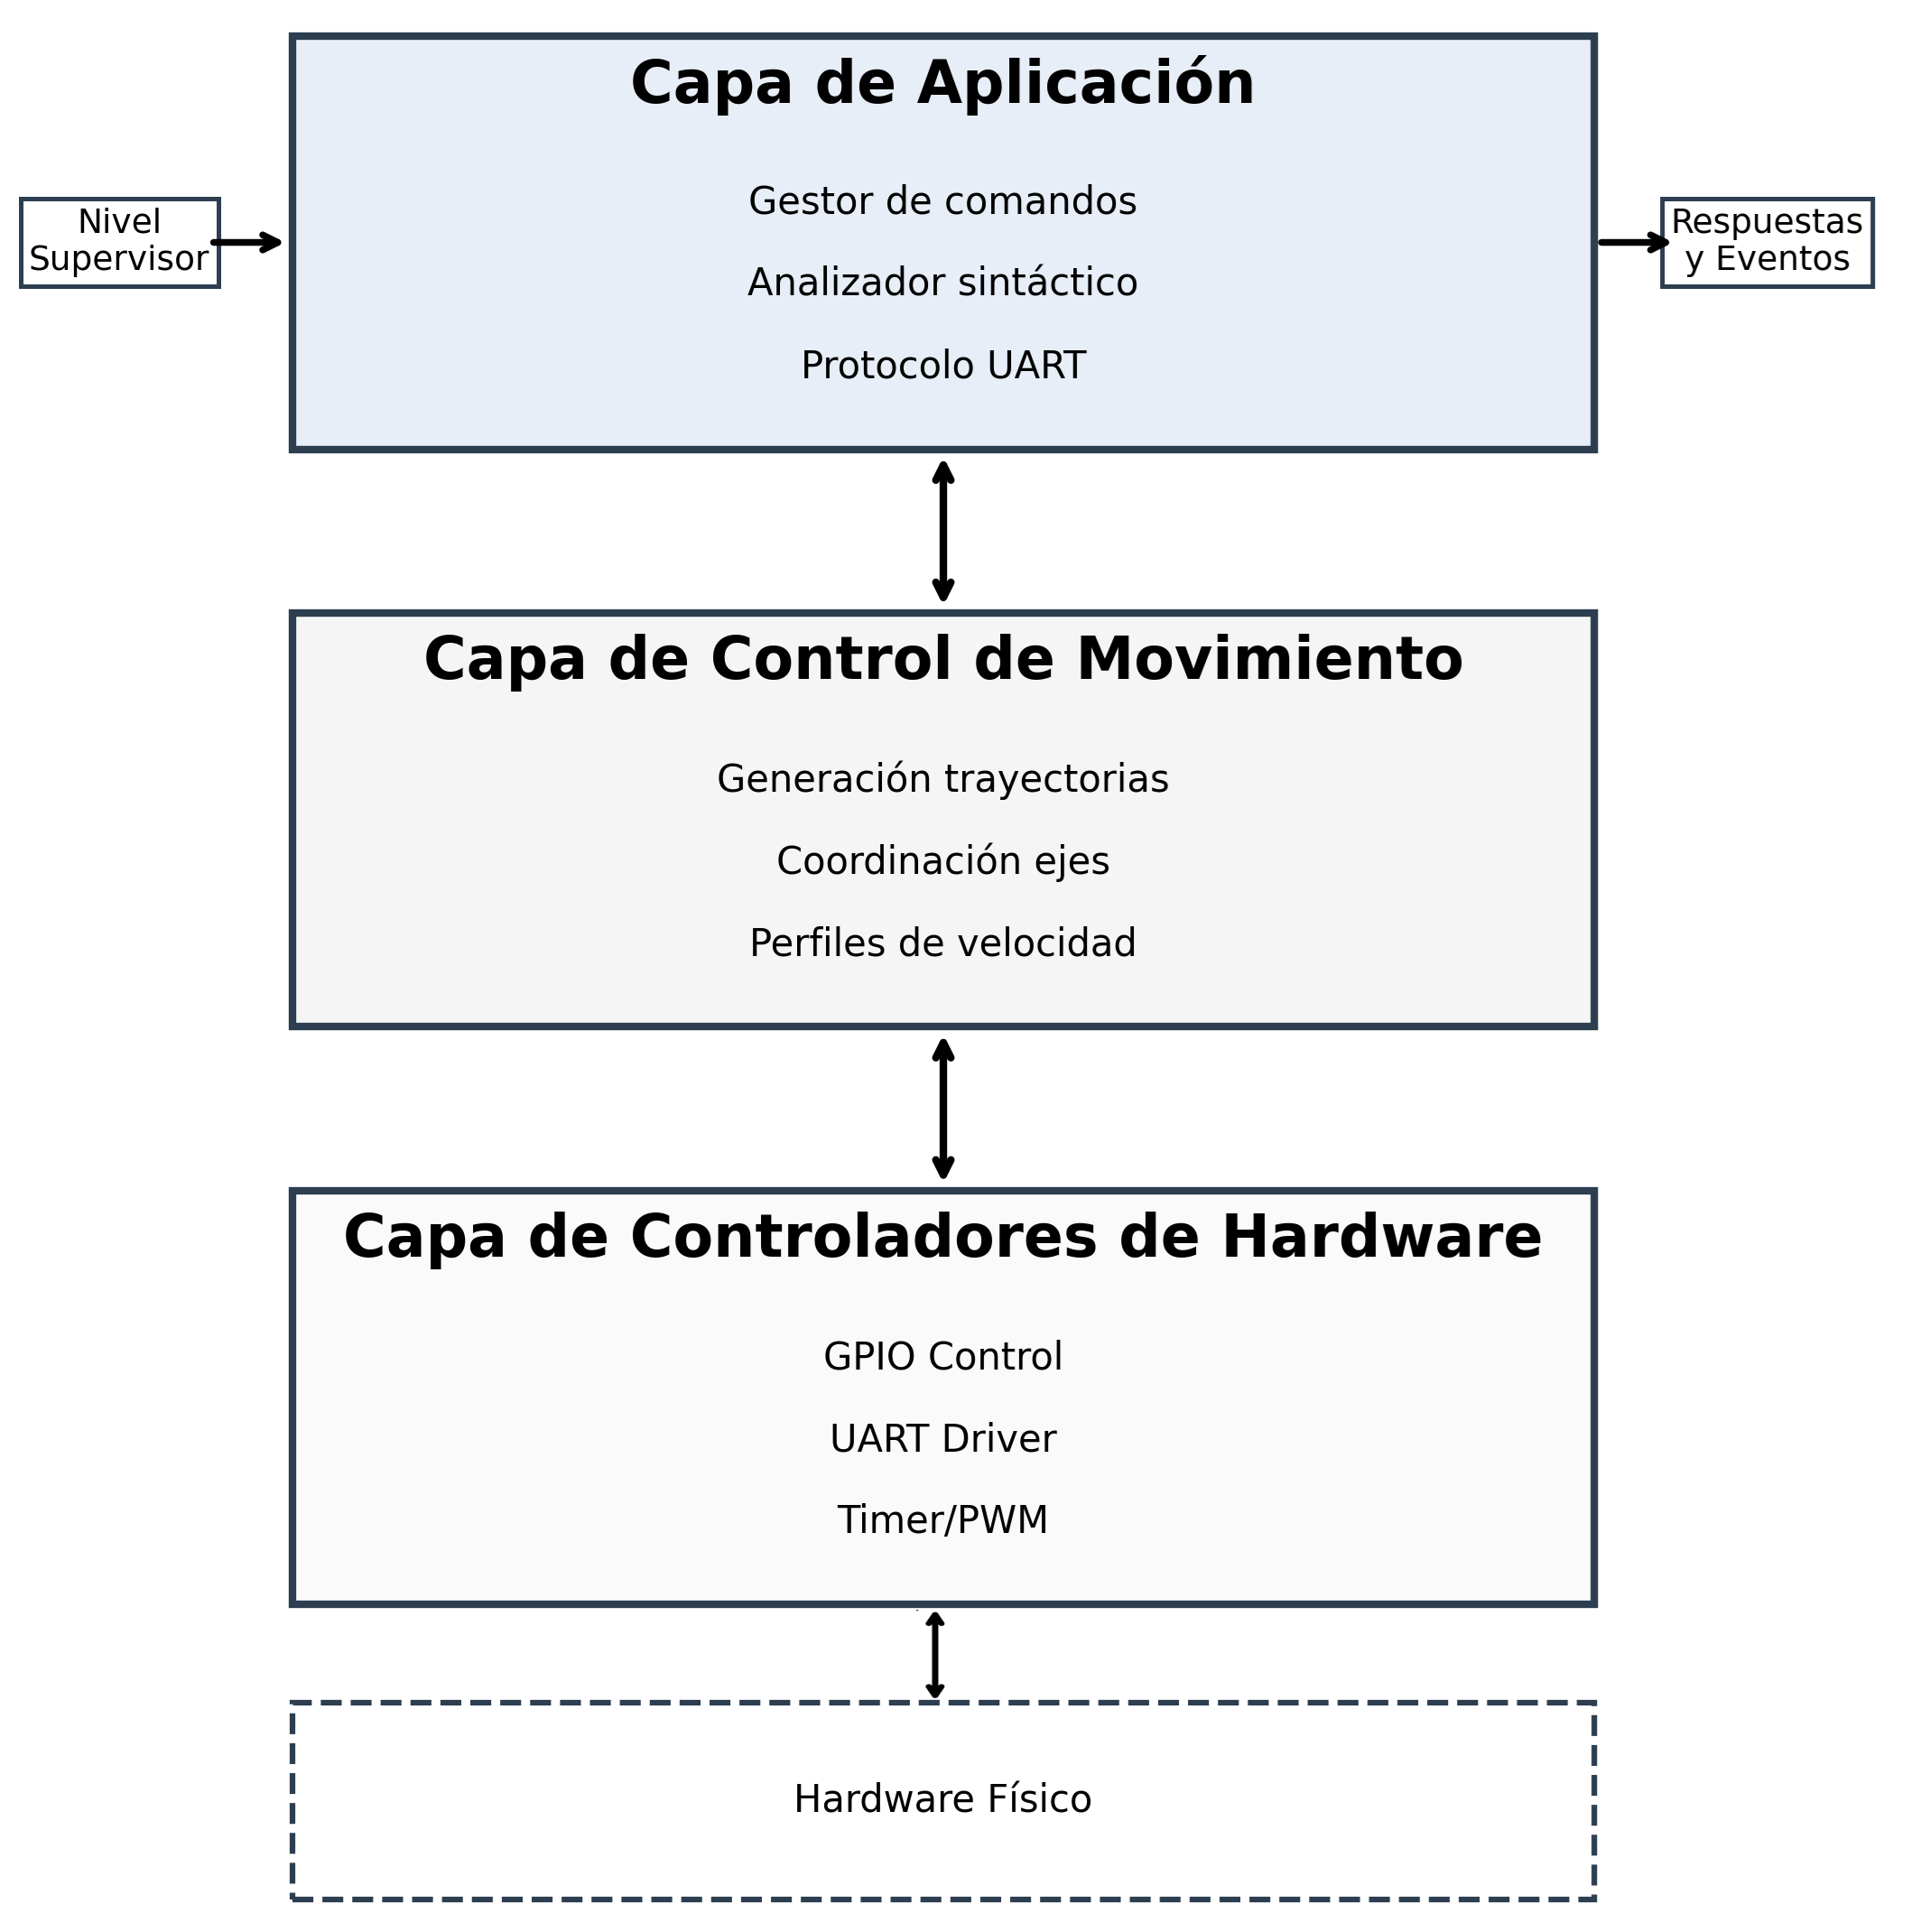
\includegraphics[width=0.7\textwidth]{imagenes/arquitectura_regulatorio_capas.png}
    \caption{\textit{Arquitectura en capas del firmware del nivel regulatorio}}
    \label{fig:arquitectura_regulatorio}
\end{figure}

El flujo de procesamiento sigue la secuencia: recepción del mensaje por UART → análisis sintáctico → configuración de perfil de movimiento → generación de interrupciones → emisión de pulsos hacia drivers → notificación de finalización al supervisor.
